% !Tex program = xelatex
% !TeX spellcheck = en_US
\documentclass[UTF8]{article}
\usepackage{indentfirst}
\usepackage{graphicx} 
\usepackage{amsmath}  
\usepackage{float}   
\usepackage{listings}

\title{Discrete Mathematics Homework}
\author{Zhengren Wang \quad 2019081308021}
\date{04/23/2020 Thu }
\begin{document}
\maketitle 

\part{2.3}
\begin{description}
    \item[3]Determine whether f is a function from the set of all bit
strings to the set of integers 

        a) False \quad
        b) True \quad
        c) False \quad
    \item[9]Find these values

        a) 1 \quad
        b) 0 \quad
        c) 0 \quad
        d) -1

        e) 3 \quad
        f) -1 \quad
        g) 2 \quad
        h) 1
    \item[15]Determine whether the function f : Z × Z → Z is onto

        a) True \quad
        b) False \quad
        c) True \quad
        d) False \quad

        e) True\quad
    \item[31]Let f (x) = $\lfloor x^2/3 \rfloor$. Find f (S)

        a) \{1,0,3\} \quad
        b) \{0,1,3,5,8\} \quad
        c) \{0,8,16,40\} \quad
        d) \{1,12,33,65\}
    \item[43]Let g(x) = $\lfloor x \rfloor$. Find
        
        a)$[0,1)$ \quad
        b)$[-1,2)$ \quad
        c)$\emptyset$ \quad

    \item[65]Draw the graph of the function f (x) = $\lfloor x \rfloor$+ $\lfloor x/2 \rfloor$ from
R to R.\\
        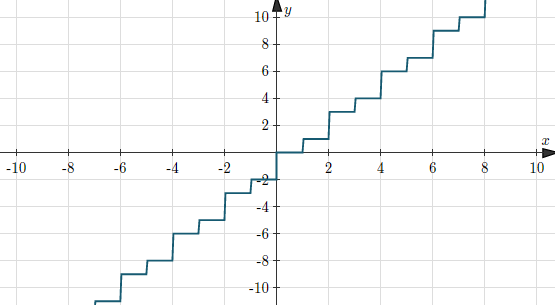
\includegraphics[scale=0.4]{../imgs/floor.png}\\
        This graph is ploted by myself, however there is some mistake, so I put this graph. \\
        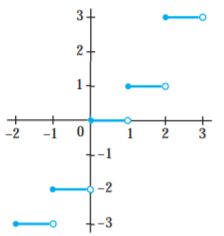
\includegraphics[scale=0.4]{../imgs/floor1.png}\\


    \item[73]Prove or disprove each of these statements about the floor
and ceiling functions.

        a) True floor(x) is always integer, ans ceiling(integer) is itself\\
        b) False (counter example : 0.5) \\
        c) True  \\
        if x or y is an integer, it's easy to see. When  both of them aren't integers, then $x = n+a$  and $y = m +b$,
where n and m are integers and a and b are less than 1 while greater than zero. Then $m+n<x+y<m+n+2$, so
$\lceil x +y \rceil$ is either m+n+1 or m+n+2. Then, the given expression is either $(n + 1) + (m + 1) − (m + n + 1) = 1$ or
$(n + 1) + (m + 1)−(m+n+2) = 0$. \\
        d) False (counter example : x=-1.1 y=-1.1) \\
        e) False (counter example : x=0.1)
\end{description}

\end{document}
